\subsection{Árboles de decisión y bosques aleatorios.}
\begin{frame}{Métodos supervisados}
\begin{columns}
\begin{column}{0.9\textwidth}
\begin{defi}
Los árboles de decisión son conjuntos de reglas discriminantes que fraccionan el espacio de observaciones en regiones donde se modeliza la variable respuesta de manera sencilla. En el proceso de ajuste generan un grafo de tipo árbol con un nodo raíz y los nodos hoja representan cada una de las regiones resultantes. 
\end{defi}
\end{column}
\end{columns}
\end{frame}

\begin{frame}{Métodos supervisados}
\begin{columns}
\begin{column}{0.9\textwidth}
Conceptos importantes:
\begin{itemize}
\item Partición de indices $(j,s)$.
\item Nodo terminal o nodo hoja.
\item Nodo padre y nodo hijo.
\item Profundidad y tamaño del árbol.
\end{itemize}
\begin{center}
\begin{figure}[ht]
  \subfloat[División de $\mathbb{R}^p$]{
   \label{f:división}
    \includegraphics[width=0.25\textwidth]{Documentos Extra/Imagenes/Regiones árboles.png}}
  \subfloat[Diagrama resultante]{
   \label{f:diagrama arbol}
    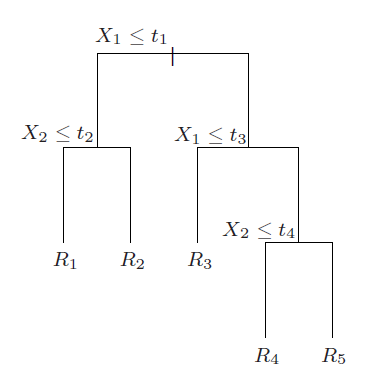
\includegraphics[width=0.25\textwidth]{Documentos Extra/Imagenes/Diagrama de arbol.png}}
 \caption{Representación de la división de $\mathbb{R}^p$ y el diagrama de árbol \\resultante.}
 \label{f:MARC1}
\end{figure}
\end{center}
\end{column}
\end{columns}
\end{frame}

\begin{frame}{Métodos supervisados}
\begin{columns}
\begin{column}{0.9\textwidth}
\textbf{Árboles de regresión}

Sea el caso en el que la variable respuesta es cuantitiva y las variables predictoras son cuantitativas o cualitativas.

Tras haber ajustado el árbol hasta tener un tamaño $|T|=M$ resultando en las regiones $R_1,\ldots, R_M$. Entonces el predictor será el siguiente: 
\begin{equation}
\hat{f}(\mathbf{x})=\sum_{m=1}^M \hat{c}_m\cdot \mathbf{1}_m(\mathbf{x})
\end{equation}
donde $\mathbf{1}_m(\mathbf{x})$ es la función característica de la región $R_m,\enspace \forall m=1,\ldots, M$. Y la constante $\hat{c}_m$ es la media de la variable respuesta en la región $R_m$.
\end{column}
\end{columns}
\end{frame}



\begin{frame}{Métodos supervisados}
\begin{columns}
\begin{column}{0.9\textwidth}
\textbf{Árboles de regresión}

Una partición $(j,s)$ que particione el espacio en las dos regiones $R_{m_1},R_{m_2}$ es elegida si minimiza la siguiente cantidad:
\begin{equation}
\sum_{i/\mathbf{x}_i\in R_{m_1} } (y_i-\hat{c}_{m_1})^2+\sum_{i/\mathbf{x}_i\in R_{m_2} } (y_i-\hat{c}_{m_2})^2
\end{equation}
\end{column}
\end{columns}
\end{frame}

\begin{frame}{Métodos supervisados}
\begin{columns}
\begin{column}{0.9\textwidth}
\textbf{Árboles de regresión}

Se puede definir la medida de bondad de ajuste a los datos de un determinado árbol de la siguiente manera:
\begin{equation}
Q(T)=\sum_{m=1}^M\frac{1}{N_m}\sum_{i/\mathbf{x}_i\in R_m} (y_i-\hat{c}_m)^2,
\end{equation}

Si se hace demasiado grande el árbol, se puede dar una situación de sobreajuste, en la que el error medio cuando se ajuste sea pequeño pero que el modelo pierda capacidad predictiva. 

\end{column}
\end{columns}
\end{frame}

\begin{frame}{Métodos supervisados}
\begin{columns}
\begin{column}{0.9\textwidth}
\textbf{Árboles de regresión}
\begin{defi}
Se llama poda al proceso en el que dado un árbol inicial de tamaño $T_0$ se revierten ciertas particiones terminales que no aportan en la relación coste-complejidad, es decir, aumentan demasiado la complejidad (aumentando la varianza), sin reducir el coste en exceso. 
\end{defi}

Se puede añadir un término regularizador para el error cuadrático.
\begin{equation}
Q_{\alpha}(T)=\sum_{m=1}^M\frac{1}{N_m}\sum_{i/\mathbf{x}_i\in R_m} (y_i-\hat{c}_m)^2+\alpha|T |,
\end{equation}
\end{column}
\end{columns}
\end{frame}


\begin{frame}{Métodos supervisados}
\begin{columns}
\begin{column}{0.9\textwidth}
\textbf{Árboles de clasificación}

Sea las variables predictoras como antes, pero la variable respuesta ahora es cualitativa. Supóngase que puede tomar $L$ valores distintos que llamaremos $l,\enspace l=1,\ldots, L$. 

\begin{equation}
\hat{p}_{lm}=\text{Proporción de observaciones en las que $y_i=l$, en la región $R_m$.}
\end{equation}
\end{column}
\end{columns}
\end{frame}

\begin{frame}{Métodos supervisados}
\begin{columns}
\begin{column}{0.9\textwidth}
\textbf{Árboles de clasificación}

Teniendo en cuenta esto se define lo siguiente:
\begin{itemize}
\item Impureza de un nodo; $1-\max_{l\in L} \hat{p}_{lm}$
\item Índice Gini $G=\sum_{l=1}^L\hat{p}_{lm}(1-\hat{p}_{lm})$
\item Entropía de un nodo $H(\hat{p}_{lm})=-\hat{p}_{lm}log(\hat{p}_{lm})-(1-\hat{p}_{lm})log(1-\hat{p}_{lm})$
\item Ganancia $Ganancia=H(padre)-\sum_{i=1}^k \dfrac{N_i}{N_{padre}}H_i,1$
\item Ratio de ganancia $\dfrac{Ganancia}{H_{padre}}$
\end{itemize}
\end{column}
\end{columns}
\end{frame}

\begin{frame}{Métodos supervisados}
\begin{columns}
\begin{column}{0.9\textwidth}
\textbf{Árboles}

Los distintos métodos de elección de las particiones dan lugar a los distintos algoritmos:
\begin{itemize}
\item \emph{CART} de Breiman para árboles tanto de regresión como de clasificación. 
\item  \emph{C.4.5} de Quinlan también para cualquier modalidad 
\item \emph{CHAID} de Kass únicamente para árboles de clasificación. 
\end{itemize}
 
\end{column}
\end{columns}
\end{frame}

\begin{frame}{Métodos supervisados}
\begin{columns}
\begin{column}{0.9\textwidth}
\textbf{Sesgo y varianza de un modelo}

\begin{defi}
Se llama error de predicción esperado de la observación $\mathbf{x}_0$ a la siguiente expresión:
\begin{equation}
EPE(\mathbf{x}_0)=\mathbb{E}((Y-\hat{f}(\mathbf{x}_0))^2)
\end{equation}
\end{defi}

\begin{propo}
El error de predicción esperado se puede dividir en un termino irreducible, el sesgo del modelo y la varianza:
\begin{equation}
EPE(\mathbf{x}_0)=Sesgo(\hat{f}(\mathbf{x}_0))^2+Var(\hat{f}(\mathbf{x}_0))
\end{equation}
\noindent donde el $Sesgo(\hat{f}(\mathbf{x}_0))=\mathbb{E}(\hat{f}(\mathbf{x}_0))-f(\mathbf{x}_0)$.
\end{propo}
\end{column}
\end{columns}
\end{frame}

\begin{frame}{Métodos supervisados}
\begin{columns}
\begin{column}{0.9\textwidth}
\textbf{Sesgo y varianza de un modelo}
\begin{center}

\begin{figure}[h]
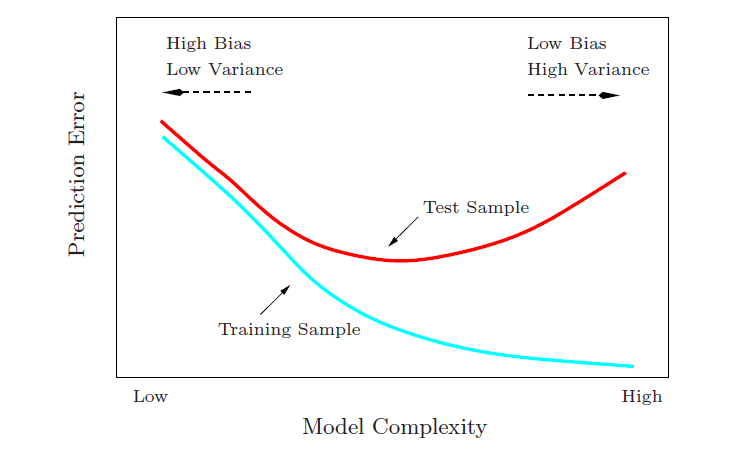
\includegraphics[scale=0.45]{Documentos Extra/Imagenes/Bias-Variance-Tradeoff.png}
\caption{Balance sesgo varianza}
\label{fig:Balance-sesgo-varianza}
\end{figure}
\end{center}
\end{column}
\end{columns}
\end{frame}

\begin{frame}{Métodos supervisados}
\begin{columns}
\begin{column}{0.9\textwidth}
\textbf{Bosques Aleatorios}

Los bosques aleatorios es un  técnica que definió Breiman. Este proceso busca hacer crecer varios árboles de manera totalmente aleatoria concretamente: 
\begin{itemize}
\item En cada árbol se utiliza una muestra aleatoria sin reemplazamiento del conjunto de datos iniciales. 
\item Se establece un número $j_{try}$ por el usuario. Para cada partición a realizar se escogen de manera aleatoria $j_{try}$ variables y se elige la que más se ajusta al criterio dado. Y se hace crecer el árbol hasta que se da un criterio de parada. 
 
\item Una vez crecidos los árboles, se toma como predicción de una nueva observación la media de las predicciones de los datos en el caso de que la variable respuesta sea continua. En el caso contrario, se toma el voto por mayoría. 
\end{itemize} 
\end{column}
\end{columns}
\end{frame}

